\subsection{模}

设 \(\mu\) 是 G 上的左哈尔测度。对于每个 \(s \in \mathbf{G}\)，\(\pmb{\delta}(s)\mu\) 也是左不变的（No.~1, 公式 (11)），因此由定理 1，存在唯一的数 \(\Delta_{\mathbf{G}}(s) > 0\)，使得 \(\pmb{\delta}(s)\mu = \Delta_{\mathbf{G}}(s)\mu\)。根据定理 1，数 \(\Delta_{\mathbf{G}}(s)\) 与 \(\mu\) 的选择无关。

定义 3. --- 函数 \(\Delta_{\mathbf{G}}\) 定义在 \(\mathbf{G}\) 上，称为 \(\mathbf{G}\) 的模（或模函数）。若 \(\Delta_{\mathbf{G}} = 1\)，则称群 \(\mathbf{G}\) 为幺模群。

也可以说 \(\mu\) 是右相对不变的，乘子为 \(\Delta_{\mathbf{G}}\)。因此 \(\Delta_{\mathbf{G}}\) 是 \(\mathbf{G}\) 在 \(\mathbf{R}_{+}^{*}\) 中的连续表示（No.~1, Prop. 1）。

评注。--- 若 \(\varphi\) 是从 \(G\) 到局部紧群 \(G'\) 的同构，则 \(\Delta_{G'} \circ \varphi = \Delta_G\)。特别地：

\begin{enumerate}
\def\labelenumi{\arabic{enumi})}
\item
  由于 \(x \mapsto x^{-1}\) 是从 \(G\) 到对立群 \(G^0\) 的同构，有 \(\Delta_{G^0} = \Delta_{G}^{-1}\)。
\item
  若 \(\varphi\) 是 \(G\) 的自同构，则 \(\Delta_G \circ \varphi = \Delta_G\)。
\end{enumerate}

取 \(s \in G\)。则：

\[
\boldsymbol {\delta} (s) \left(\Delta_ {\mathrm{G}} ^ {- 1} \cdot \mu\right) = \left(\boldsymbol {\delta} (s) \Delta_ {\mathrm{G}} ^ {- 1}\right) \cdot \left(\boldsymbol {\delta} (s) \mu\right) = \left(\Delta_ {\mathrm{G}} (s) ^ {- 1} \Delta_ {\mathrm{G}} ^ {- 1}\right) \cdot \left(\Delta_ {\mathrm{G}} (s) \mu\right) = \Delta_ {\mathrm{G}} ^ {- 1} \cdot \mu ,
\]

因此 \(\Delta_{\mathrm{G}}^{-1} \cdot \mu = \mu'\) 是右哈尔测度。由此可得 \(\boldsymbol{\gamma}(s)\mu' = (\boldsymbol{\gamma}(s)\Delta_{\mathrm{G}}^{-1}) \cdot \mu = \Delta_{\mathrm{G}}(s)(\Delta_{\mathrm{G}}^{-1} \cdot \mu) = \Delta_{\mathrm{G}}(s)\mu'\)，所以对于每个右哈尔测度 \(\nu\)，都有 \(\boldsymbol{\gamma}(s)\nu = \Delta_{\mathrm{G}}(s)\nu\)。由于 \(\breve{\mu}\) 是右哈尔测度，有 \(\breve{\mu} = a\Delta_{\mathrm{G}}^{-1} \cdot \mu\)，其中常数 \(a > 0\)；于是

\[
\mu = a \big (\Delta_ {\mathrm{G}} ^ {- 1} \cdot \mu \big) ^ {\vee} = a \Delta_ {\mathrm{G}} \cdot \stackrel {\vee} {\mu} = a ^ {2} \mu ,
\]

因此 \(a = 1\)，最后 \(\check{\mu} = \Delta_{\mathrm{G}}^{-1}\cdot \mu\)。同理可得 \(\check{\nu} = \Delta_{\mathrm{G}}\cdot \nu\)。因此有以下结果：

公式表。--- 设 G 是局部紧群，\(\Delta\) 是其模，\(\mu\) 是左哈尔测度，\(\nu\) 是右哈尔测度。

\begin{enumerate}
\def\labelenumi{\arabic{enumi})}
\tightlist
\item
  有
\end{enumerate}

\[
\boldsymbol {\gamma} (s) \mu = \mu \quad \boldsymbol {\delta} (s) \mu = \Delta (s) \mu \quad \check {\mu} = \Delta^ {- 1} \cdot \mu .\tag{20}
\]

若 \(f\) 在 \(\mu\) 下于 \(G\) 可积，则 \(f\) 的左、右平移也在 \(\mu\) 下可积，并且

\[
\begin{array}{l} \int f (s x) d \mu (x) = \int f (x) d \mu (x) \\ \int f (x s) d \mu (x) = \Delta (s) ^ {- 1} \int f (x) d \mu (x). \end{array}\tag{21}
\]

此外，\(\stackrel{\vee}{f}\) 对 \(\Delta^{-1} \cdot \mu\) 可积，并且

\[
\int f (x ^ {- 1}) \Delta (x) ^ {- 1} d \mu (x) = \int f (x) d \mu (x).\tag{22}
\]

若 A 是 G 的 \(\mu\)-可积子集，则 sA 和 As 也在 \(\mu\) 下可积，并且

\[
\mu (s \mathrm{A}) = \mu (\mathrm{A}) \quad \mu (\mathrm{A} s) = \Delta (s) \mu (\mathrm{A}).\tag{23}
\]

\begin{enumerate}
\def\labelenumi{\arabic{enumi})}
\setcounter{enumi}{1}
\tightlist
\item
  有
\end{enumerate}

\[
\boldsymbol {\delta} (s) \nu = \nu \quad \boldsymbol {\gamma} (s) \nu = \Delta (s) \nu \quad \check {\nu} = \Delta \cdot \nu .\tag{24}
\]

若 \(f\) 在 \(\nu\) 下于 \(G\) 可积，则 \(f\) 的左、右平移也在 \(\nu\) 下可积，并且

\[
\begin{array}{l} \int f (x s) d \nu (x) = \int f (x) d \nu (x) \\ \int f (s x) d \nu (x) = \Delta (s) \int f (x) d \nu (x). \end{array}\tag{25}
\]

此外，\(\stackrel{\vee}{f}\) 对 \(\Delta \cdot \nu\) 可积，并且

\[
\int f (x ^ {- 1}) \Delta (x) d \nu (x) = \int f (x) d \nu (x).\tag{26}
\]

若 A 是 G 的 \(\nu\)-可积子集，则 sA 和 As 也在 \(\nu\) 下可积，并且

\[
\nu (\mathrm{A} s) = \nu (\mathrm{A}) \quad \nu (s \mathrm{A}) = \Delta (s) ^ {- 1} \nu (\mathrm{A}).\tag{27}
\]

\begin{enumerate}
\def\labelenumi{\arabic{enumi})}
\setcounter{enumi}{2}
\item
  \(\nu\) 与 \(\Delta^{-1} \cdot \mu\) 成比例，且 \(\mu\) 与 \(\Delta \cdot \nu\) 成比例。
\item
  假设 G 是幺模的。令 \(\mu\) 为 G 上的哈尔测度。则：
\end{enumerate}

\[
\boldsymbol {\gamma} (s) \mu = \boldsymbol {\delta} (s) \mu = \stackrel {\vee} {\mu} = \mu .\tag{28}
\]

若 \(f\) 在 \(\mu\) 下于 \(G\) 可积，则 \(f\) 的左、右平移也在 \(\mu\) 下可积，\(\overset{\vee}{f}\) 亦然，并且

\[
\int f (s x) d \mu (x) = \int f (x s) d \mu (x) = \int f (x ^ {- 1}) d \mu (x) = \int f (x) d \mu (x).\tag{29}
\]

若 \(\mathbf{A}\) 是 \(\mu\) 下在 \(\mathbf{G}\) 中可积的子集，则 \(s\mathbf{A}\)、\(\mathbf{A}s\) 和 \(\mathbf{A}^{-1}\) 都在 \(\mu\) 下可积，并且

\[
\mu (s \mathrm{A}) = \mu (\mathrm{A} s) = \mu (\mathrm{A} ^ {- 1}) = \mu (\mathrm{A}).\tag{30}
\]

本质积分也具有相应的性质。

命题 3. --- 若 G 中存在一个在内自同构下不变的 e 的紧邻域 V，则 G 是幺模的。

事实上，设 \(\mu\) 是 \(\mathbf{G}\) 上的左哈尔测度。对于每个 \(s \in \mathbf{G}\)，

\[
\mu (\mathrm{V}) = \mu (s ^ {- 1} \mathrm{Vs}) = \Delta_ {\mathrm{G}} (s) \mu (\mathrm{V}),
\]

从而 \(\Delta_{\mathbf{G}}(s) = 1\)，因为 \(0 < \mu (\mathrm{V}) < +\infty\)。

由此立即得到：

推论。--- 若 G 是离散的、紧的或交换的，则 G 是幺模的。

当 G 交换时，这一点更是显然的。还要注意，若 G 是离散的，则 G 上每个点质量为 1 的测度显然是 G 上的左、右哈尔测度，称为 G 上的归一化哈尔测度。若 G 是紧的，则 G 上存在唯一满足 \(\mu(G)=1\) 的哈尔测度，称为 G 的归一化哈尔测度。当前两种约定同时适用于 G 既离散又紧、即有限的情形时，它们并不一致；在这种情况下，我们总会明确说明“归一化哈尔测度”的含义。

\pandocbounded{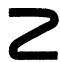
\includegraphics[keepaspectratio]{images/part001_35d0c9a3.jpg}}

幺模群的子群和商群不一定幺模（\(\S2\)，习题 5）。不过参见 \(\S2\) 的命题 10, No.~7。

*稍后我们将看到，半单或幂零连通李群是幺模的。*

